% Enable warnings about problematic code
\RequirePackage[l2tabu, orthodox]{nag}

\documentclass{WeSTassignment}

% The lecture title, e.g. "Web Information Retrieval".
\lecture{Introduction to Web Science}
% The names of the lecturer and the instructor(s)
\author{%
  Mohammad Nizam Uddin\\{\normalsize{216101140}} \and
  Syed Nabil Afaraz Bukhari\\{\normalsize{216100868}} 
}
% Assignment number.
\assignmentnumber{1, Group: " Lima "}



% Institute of lecture.
\institute{%
  Institute of Web Science and Technologies\\%
  Department of Computer Science\\%
  University of Koblenz-Landau%
}
% Date until students should submit their solutions.
\datesubmission{November 2, 2016, 10:00 a.m.}
% Date on which the assignments will be discussed in the tutorial.
\datetutorial{November 4th, 2016, 12:00 p.m.}

% Set langauge of text.
\setdefaultlanguage[
  variant = american, % Use American instead of Britsh English.
]{english}

% Specify bib file location.
\addbibresource{bibliography.bib}

% For left aligned centerd boxes
% see http://tex.stackexchange.com/a/25591/75225
\usepackage{varwidth}

% ==============================================================================
% Document

\begin{document}

\maketitle

The main objective of this assignment is for you to use different tools with which you can understand the network that you are connected to or you are connecting to in a better sense.
These tasks are not always specific to \enquote{Introduction to Web Science}.
For all the assignment questions that require you to write a code, make sure to include the code in the answer sheet, along with a separate python file. Where screen shots are required, please add them in the answers directly and not as separate files. 

% As such, this assignment will not award any points, and you will \emph{not} have
% to submit your solution.
% If you want to know whether your solutions were correct, mail them to
% \mailto{lukas@uni-koblenz.de}.

% ------------------------------------------------------------------------------

\section{Ethernet Frame (5 Points)}

Ethernet Frame is of the given structure:
\begin{figure}[h]
  \centering
  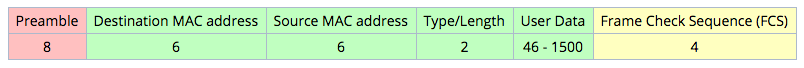
\includegraphics[width=0.9\textwidth]{1.png}
   \caption{Ethernet Frame Structure}
     \label{fig:ethernet}
\end{figure}

Given below is an Ethernet frame without the Preamble and the Frame Check Sequence.\\ 
 
\texttt{00 27 10 21 fa 48 00 13 \hspace{0.5cm} 10 e8 dd 52 08 06 00 01\\ 08 00 06 04 00 01 00 13 \hspace{0.5cm} 10 e8 dd 52 c0 a8 02 01\\ 00 00 00 00 00 00 c0 a8 \hspace{0.5cm} 02 67} \\ \\

\underline{Find}:
\begin{enumerate}
\item Source MAC Address
\item Destination MAC Address
\item What protocol is inside the data payload?
\item Please mention what the last 2 fields hold in the above frame.\\ \\
\end{enumerate}




\paragraph{\underline{Answer:}}
\begin{enumerate}
\item According to the frame given the Source MAC address is 00:13:10:e8:dd:52
\item The Destination MAC address is 00:27:10:21:fa:48
\item The protocol is Advance Resolution Protocol inside the data payload because the Ether-type is 0x 08 06
\item In the above frame the last two fields are the target hardware address and target IP address. According to the frame the target hardware address is 00:00:00:00:00:00 and the target IP address is c0:a8:02:67
\end{enumerate}
% ------------------------------------------------------------------------------

\section{Cable Issue (5 Points)}

Let us consider we have two cables of 20 meters each. One of them is in a 100MBps network while the other is in a 10MBps network. If you had to transfer data through each of them, how much time it would take for the first bit to arrive in each setting? (For your calculation you can assume that the speed of light takes the same value as in the videos.) Please provide formulas and calculatoins along with your results. \\ \\

\paragraph{\underline{Answer:}}
\begin{enumerate}
\item In a 100MBps network to transfer first bit of data it takes 10 nanosecond to go a distance of 3 meters. So to travel 20 meters it would take (10*20)/3 = 66.67 ns
\item In a 10MBps network to transfer first bit of data it takes 100 nanosecond to go a distance of 30 meters. So to travel 20 meters it would take (100*20)/30 = 66.67 ns
\end{enumerate}



% ------------------------------------------------------------------------------


\section{Basic Network Tools (10 Points)}

Listed below are some of the commands which you need to "google" to understand what they stand for:
\begin{enumerate}
\item \emph{ipconfig / ifconfig}
\item \emph{ping}
\item \emph{traceroute}
\item \emph{arp}
\item \emph{dig}
\end{enumerate}

Consider a situation in which you need to check if \url{www.wikipedia.org} is reachable or not. Using the knowledge you gained above to \underline{find the following information}:
\begin{enumerate}
\itemsep0em
\item The \emph{\% packet loss} if at all it happened after sending 100 packets. 
\item \emph{Size} of the packet sent to \emph{Wikipedia} server
\item \emph{IP address} of your machine and the \emph{Wikipedia} server
\item \emph{Query Time} for DNS query of the above url.
\item Number of \emph{Hops} in between your machine and the server
\item MAC address of the device that is acting as your network gateway. 
\end{enumerate}

Do this once in the university and once in your home/dormitory network. With your answers, you must paste the screen shots to validate your find.\\

\underline{\textbf{Answer:}}\\ \\
%----------------------- 1 --------------------
\textrm{1. Checking the amount of packet loss in 100 packets sent to www.wikipedia.org}\\ \\
\textbf{Home Network:\\}
0.0\% packet loss. Command ( ping -c 100 www.wikipedia.org )\\
\textbf{University Network:\\}
0.0\% packet loss. Command ( ping -c 100 www.wikipedia.org )\\ 
\begin{figure}[bp!]
  \centering
  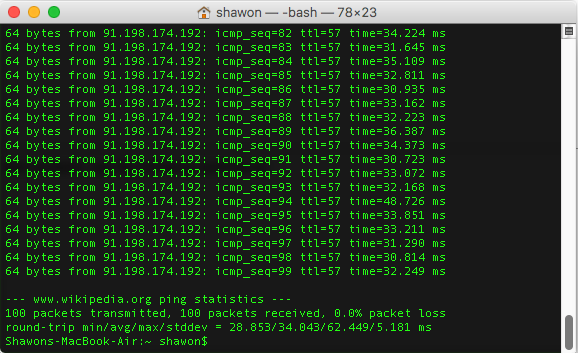
\includegraphics[width=0.9\textwidth]{home_ping.png}
   \caption{Packet loss count Home Network}
     \label{fig:packetloss}
\end{figure}
\begin{figure}[bp!]
  \centering
  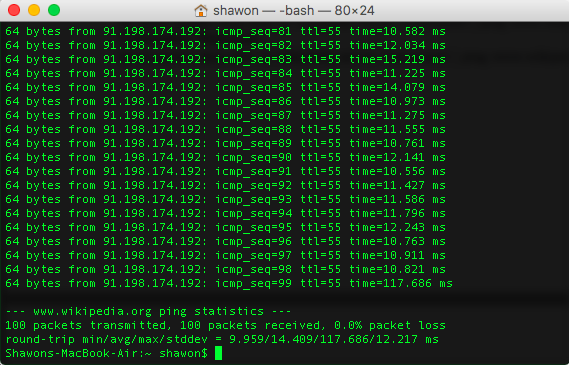
\includegraphics[width=0.9\textwidth]{uni_ping.png}
   \caption{Packet loss count University Network}
     \label{fig:packetloss}
\end{figure}\\
%------------------------ 2 --------------------
\textrm{2. Checking the packet size sent to wikipedia server}\\ \\
\textbf{Home Network:\\}
56 bytes packet data sent to wikipedia server. Command ( ping www.wikipedia.org )\\
\textbf{University Network:\\}
56 bytes packet data sent to wikipedia server. Command ( ping www.wikipedia.org )\\ \\
\begin{figure}[bp!]
  \centering
  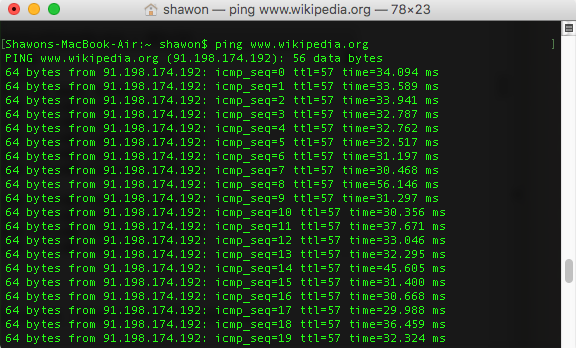
\includegraphics[width=0.9\textwidth]{home_ping1.png}
   \caption{Packet size Home Network}
     \label{fig:packetsize}
\end{figure}
\begin{figure}[bp!]
  \centering
  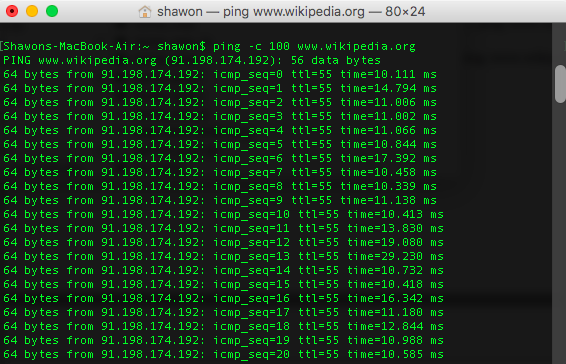
\includegraphics[width=0.9\textwidth]{uni_ping1.png} 
   \caption{Packet size University Network}
     \label{fig:packetsize}
\end{figure}
%--------------------------- 3 -----------------
\textrm{3. Finding IP address of local machine and wikipedia server}\\ \\
\textbf{Home Network:\\}
The IP address of local machine is 192.168.0.15 and wikipedia server IP is 91.198.174.192
\textbf{University Network:\\}
The IP address of local machine is 141.26.185.11 and wikipedia server IP is 91.198.174.192\\ \\
\begin{figure}[bp!]
  \centering
  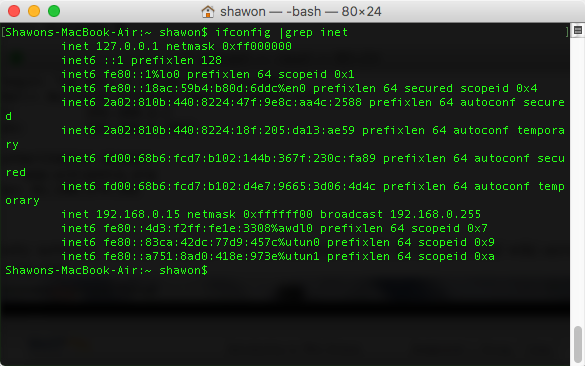
\includegraphics[width=0.9\textwidth]{home_own_ip.png}
   \caption{Local IP Home Network}
     \label{fig:ipaddress}
\end{figure}
\begin{figure}[bp!]
  \centering
  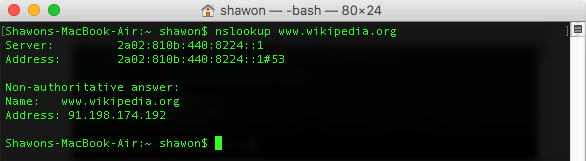
\includegraphics[width=0.9\textwidth]{home_wiki_ip.png}
   \caption{Wikipedia IP Home Network}
     \label{fig:ipaddress}
\end{figure}
\begin{figure}[bp!]
  \centering
  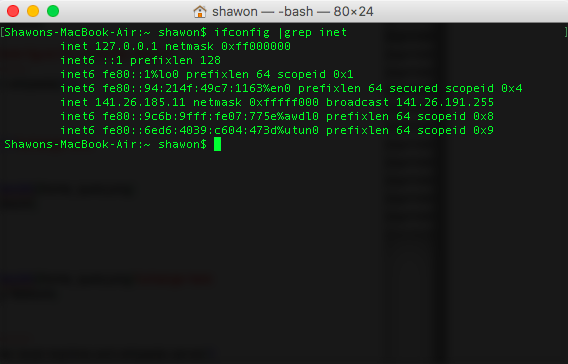
\includegraphics[width=0.9\textwidth]{uni_own_ip.png}
   \caption{Local IP University Network}
     \label{fig:ipaddress}
\end{figure}
\begin{figure}[bp!]
  \centering
  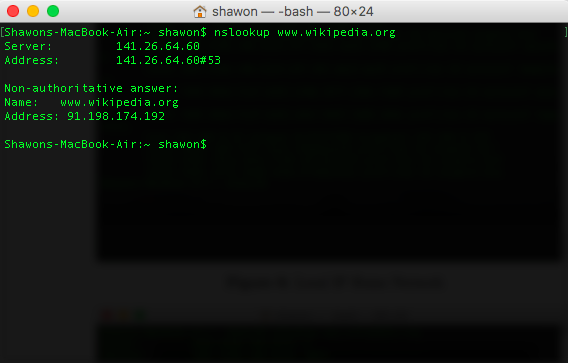
\includegraphics[width=0.9\textwidth]{uni_wiki_ip.png}
   \caption{Wikipedia IP University Network}
     \label{fig:ipaddress}
\end{figure}

%------------------------ 4 ------------------
\textrm{4. Finding query time for wikipedia}\\ \\
\textbf{Home Network:\\}
DNS query time 44 msec\\
\textbf{University network:\\}
DNS query time 73 msec\\ \\ \\ \\ \\
\begin{figure}[bp!]
  \centering
  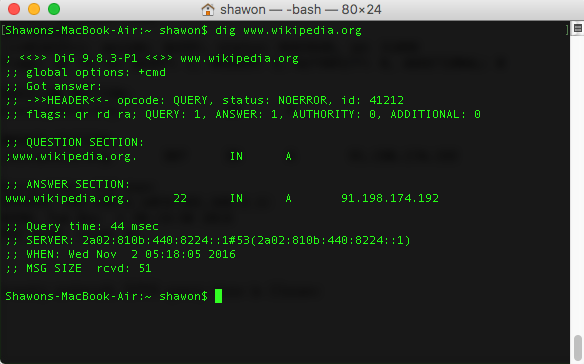
\includegraphics[width=0.9\textwidth]{home_query.png}
   \caption{DNS query Home Network}
     \label{fig:dnsquery}
\end{figure}
\begin{figure}[bp!]
  \centering
  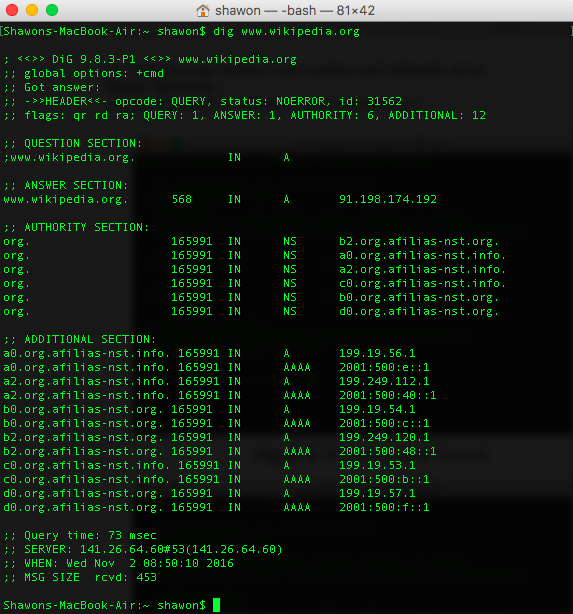
\includegraphics[width=0.9\textwidth]{uni_query.png}
   \caption{DNS query University Network}
     \label{fig:dnsquery}
\end{figure}
%----------------------- 5 --------------------
\textrm{5. Counting hops between local machine and wikipedia server}\\
\textbf{Home Network:\\}
6 hops. Command ( traceroute www.wikipedia.org )\\ \\
\textbf{University Network:\\}
8 hops. Command ( traceroute www.wikipedia.org )\\ \\ \\
\begin{figure}[bp!]
  \centering
  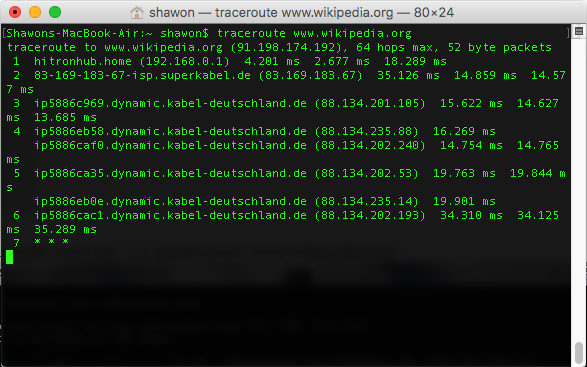
\includegraphics[width=0.9\textwidth]{home_hops.png}
   \caption{Hops count Home Network}
     \label{fig:hopscount}
\end{figure}
\begin{figure}[bp!]
  \centering
  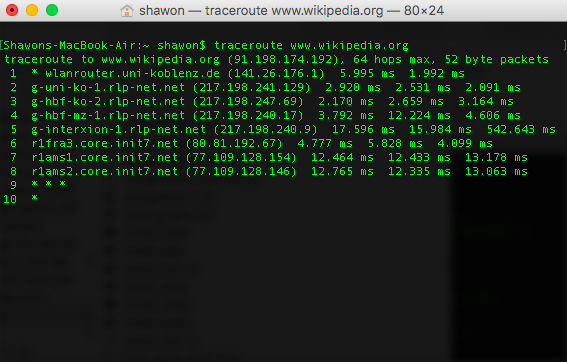
\includegraphics[width=0.9\textwidth]{uni_hops.png}
   \caption{Hops count University Network}
     \label{fig:hopscount}
\end{figure}
%---------------------6----------------------
\textrm{6. Finding network gateway MAC address}\\ \\
\textbf{Home Network:\\}
Network gateway device MAC address 68:b6:fc:d7:b1:2 Command ( arp - a )\\
\textbf{University Network:\\}
Network gateway device MAC address 14:18:77:45:b1:bd Command ( arp - a )\\ 
\begin{figure}[bp!]
  \centering
  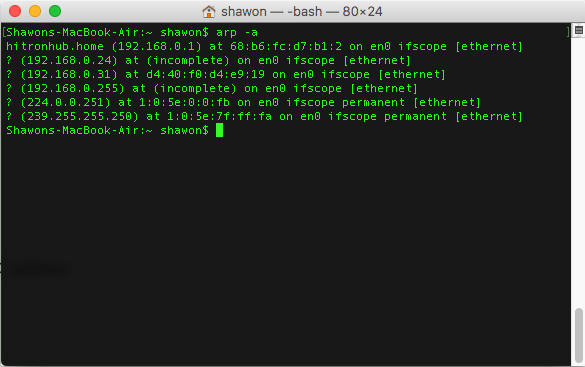
\includegraphics[width=0.9\textwidth]{home_mac.png}
   \caption{MAC address of gateway device Home Network}
     \label{fig:macaddress}
\end{figure}
\begin{figure}[bp!]
  \centering
  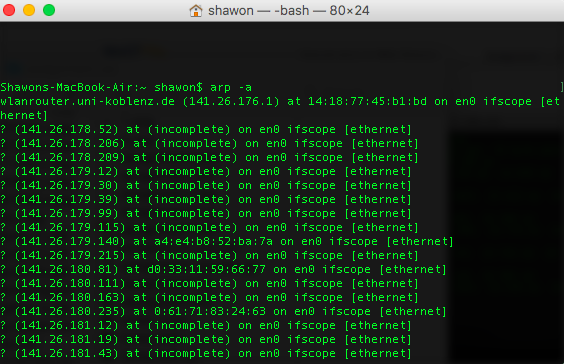
\includegraphics[width=0.9\textwidth]{uni_mac.png}
   \caption{MAC address of gateway device University Network}
     \label{fig:macaddress}
\end{figure}

% ------------------------------------------------------------------------------


\section{Simple Python Programming (10 Points)}

Write a simple \underline{python program that does the following}:
\begin{enumerate}
\item Generate a random number sequence of 10 values between 0 to 90. 
\item Perform \texttt{sine} and \texttt{cosine} operation on numbers generated. 
\item Store the values in two different arrays named SIN \& COSIN respectively. 
\item Plot the values of SIN \& COSIN in two different colors. 
\item The plot should have labeled axes and legend.
\end{enumerate}

\underline{\textbf{Answer:}}\\ \\
import numpy as nump\\
import random as rand\\
import matplotlib.pyplot as plot\\ \\
x=set()\\
for m in range(0,10):\\
	x.add(rand.randint(0,90))\\
x=sorted(x)\\
m=list(x)\\ \\
ySin = nump.sin(m)\\
yCos = nump.cos(m)\\
\#Set title and plot the graph, set green color for Sin and Red for Cos\\
plot.title('Sin and Cos functions')\\
plot.plot(x, ySin,'g' ,x,yCos,'r')\\ \\
\# Get plot axis and change y axis limits\\
x1,x2,y1,y2 = plot.axis()\\
plot.axis((x1,x2,-3,3))\\ \\
\#Add labels, legend and show the graph\\
plot.xlabel('X - Axis')\\
plot.ylabel('Y - Axis')\\
plot.legend(['Sine', 'Cosine'])\\
plot.show()\\


\makefooter

\end{document}
